\section{EVALUATION}

Our evaluation focused on PlateMate's feasibility as a replacement for traditional food logging.  We considered three broad criteria:
\vspace*{-2mm}
\begin{enumerate}
\item \textbf{Accuracy.} How accurate were crowdsourced estimates compared to current alternatives? Could users trust them?
\item \textbf{Usability.} How much effort or discomfort would users experience in photographing food, uploading the photos, and correcting errors in PlateMate's estimates?
\item \textbf{Robustness.} How well does the PlateMate system fare with ``real world'' photographs?
\end{enumerate}
\vspace*{-2mm}
We designed two experiments to answer these questions.  In the first, nutrition data returned from PlateMate was compared with ground truth, expert dietitian estimates, and a recent commercial application.  In the second study, ten participants used PlateMate and a manual food-logging system for four days.

\subsection{Evaluation of Accuracy}

Our first study had two goals. The first was to determine the accuracy of PlateMate with ground truth data obtained from manufacturers or preparers. The second was to compare PlateMate's performance with two alternative approaches to remote food photography: analysis by experts and results from Meal Snap.  
\newcontent{Because Meal Snap only returns calorie information and to make the task manageable for our expert participants, we limited our comparison to estimated calories even though PlateMate generates reports that also include fat, protein, and carbohydrates.}

\begin{figure}
\begin{center}
   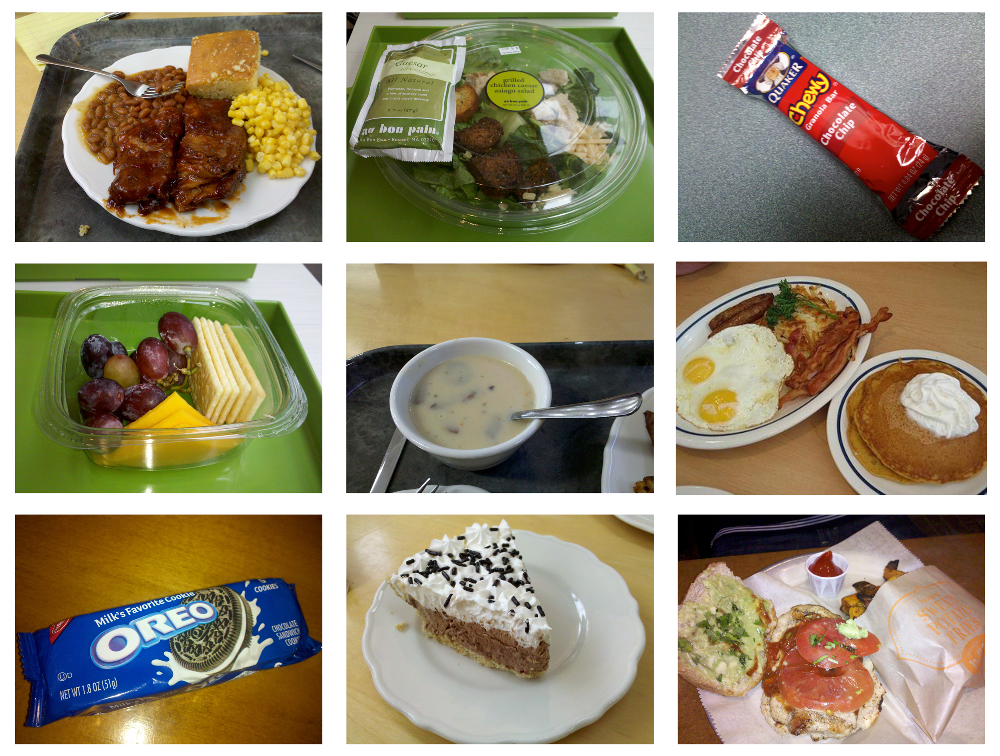
\includegraphics[width=\columnwidth]{figs/groundtruth.pdf}
   \caption{Examples of photos from the study of PlateMate's accuracy.}
   \label{fig:groundTruth}
\end{center}
\end{figure}

\subsubsection{Method}
We conducted the experiment with a sample of 18 photographs showing 36 distinct foods. Some depicted individual foods or packages, while others showed complex plates containing many items, as shown in Figure~\ref{fig:groundTruth}.  Each pictured food had nutritional data available through the manufacturer or preparer, and foods were weighed when necessary to ensure accuracy. These foods were selected to span a variety of meals and sources, including restaurants, cafeterias, and grocery items.  We also included a mix of simple foods and composite items like salads and sandwiches.

We recruited three professional dietitians to provide expert estimates: one was a private nutrition counselor, and the other two were employed by a hospital. They received compensation for their time and provided estimates from their own offices. They were encouraged to use any aids, like books and calorie databases, that they would typically use for a similar task.
% Note that their analysis is not directly comparable to the expert estimates in the original RFPM study~\cite{martin2009novel}. That experiment focused only on measuring portions, and experts were told what the foods were and provided with photographs of standard portions of each. Our study focused on genuine remote analysis, where experts had only the picture to work from. 

Our third set of estimates came from Meal Snap, a recent commercial application.  Meal Snap returns a range of calories rather than a definitive answer, so we used the mean of its high and low values.  

\begin{figure}
\begin{center}
   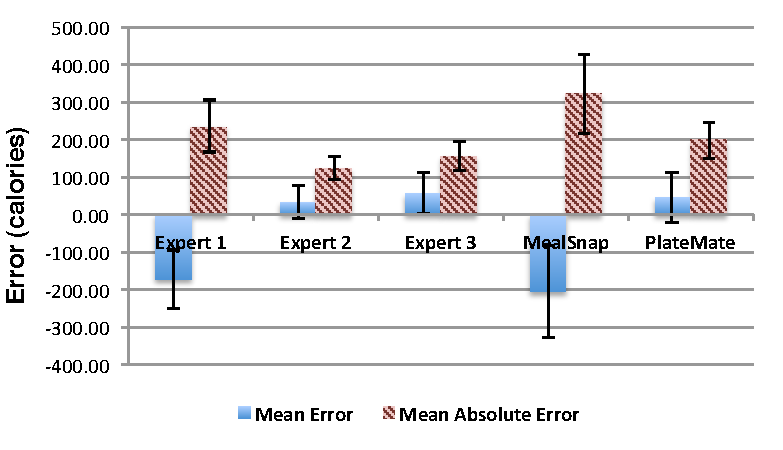
\includegraphics[width=\columnwidth]{figs/error-both}
   \caption{Mean errors (i.e., overall bias) and mean absolute errors (average magnitude of an error) for estimates made by the human experts, the Meal Snap application, and PlateMate compared to data provided by manufacturer or preparer.  Error bars correspond to standard error.}
   \label{fig:error}
\end{center}
\end{figure}

\subsubsection{Results}

In terms of mean absolute error on calorie estimates, PlateMate was not significantly different from the human experts or the Meal Snap application.  Figure~\ref{fig:error} illustrates the results in detail.  
As expected, trained dietitians were the most accurate on average. Their mean absolute error rates were $39.4\%$, $20.8\%$, and $26.1\%$, for an average of $172.0$ calories or $28.7\%$ per photograph. The best expert was off by just $124.5$ calories, on average. PlateMate was close behind with a mean absolute error rate of $198$ calories, or $33.2\%$.  MealSnap was farther behind, with an average error rate of $322.8$ calories or $53.9\%$.

Absolute error rates reflect the average magnitude of the error, but not the biases in each method. To understand how estimates from each source would add up over time, we also measured mean error without taking absolute values. The best expert overestimated by just 32.75 calories on average, for a mean error rate of $+5.5\%$.  The other two experts had error rates of $+9.2\%$ and $-27.5\%$.

%This result was in line with~\cite{martin2009novel}, which found trained nutritionists underestimated portions with an error rate of $-6.6\%$, though our task also required identifying the foods.

In comparison, PlateMate had a mean error rate of $+44.1$ calories, or $+7.4\%$, which was much closer than Meal Snap's $-34.4\%$. Expert and PlateMate results are significantly correlated with the ground truth data ($r^2 = .8626$, $.9062$, and $.9378$ for the experts, and $r^2=.8622$ for PlateMate, all with $p<.0001$), while Meal Snap results were not correlated with the actual nutritional content of the meals ($r^2=.2352$, $p=.3475$).
%MealSnap results appear almost completely uncorrelated with ground truth ($r^2=0.23$), while PlateMate and expert results were strongly correlated with actual calorie content of each food ($r^2=0.86$ and $0.93$, respectively). \bug[the $r^2$ for expert results, is this an average of the three experts?  Perhaps the better thing would be to show all three?]

%These results suggest that, while all three methods of remote food photography are somewhat inaccurate, PlateMate and experts are much better than MealSnap. MealSnap's results were almost random, while PlateMate and expert results tracked ground truth closely. PlateMate was less accurate than the best expert, but about the same as the mean.

PlateMate's error rate compares favorably to amateur self-reports, where error rates can be greater than $400$ calories/day and range from $-76\%$ to $+24\%$~\cite{schoeller1990inaccuracies,champagne2002energy}.  It also lacks the systematic bias towards underestimation in self-reports, especially among vulnerable users. These results indicate that PlateMate's answers, while imperfect, can be a useful nutritional guide.

\subsubsection{Error Analysis}

Most errors in the study corresponded to single failures in specific parts of the pipeline.   In the Tag stage, boxes were sometimes drawn improperly, leading to missing or duplicate identifications.  In one photo of a brownie and banana on a small plate, only one box was drawn covering the entire banana and most of the brownie.  As a result, the workers at the Identify stage omitted the brownie.  On a photo of a hamburger with mushrooms, overlapping boxes were drawn over the burger and topping.  In this case, the mushrooms were identified in both boxes.  

Most errors occurred in the Identify stage.  Turkers had trouble distinguishing similar types of a food, which sometimes had large nutrition differences.  A plate of vegetarian baked beans was identified as regular baked beans, tripling the calorie count.  Branded foods also caused problems: a relatively low-calorie chicken sandwich was identified as a sandwich from the restaurant Chili's, which had over twice as many calories.  Another common situation involved duplication with both a composite item and one or more foods included in that composite both being selected.  A slice of pizza with pepperoni and olives was identified as ``Pizza with Meat and Vegetables,'' ``Pepperoni,'' and ``Black Olives,'' duplicating the toppings.

During measurement, many very small quantities were overestimated, especially when a small amount of a food was spread over a large area.  A dash of parsley on a sandwich was overestimated as .27 cups, for example.  Other errors occurred when one food appeared in several boxes. This led to a hamburger bun being counted as two buns when each half of the bun was seen in its own box.

\subsection{User Study}
Our second study looked at the subjective experience of using PlateMate as an end-to-end system for nutritional monitoring, compared to manual logging.  We looked for insights about the system's usability, in terms of the inconvenience of taking photographs and the effort required to correct errors.  Finally, we wanted to observe how robustly PlateMate functioned in the ``real world,'' without any constraints on the types of photographs submitted to the system.

\subsubsection{Method}
We recruited 10 participants (4 male, 6 female) via advertisements posted on several university email lists.  Seven of the participants were undergraduates, two were graduate students, and one was a faculty member.

To help us evaluate the quality of the nutritional estimates generated by PlateMate and by the participants in this study, we recruited four dietitians employed at a local hospital.  Two of them had also participated in the experiment evaluating the accuracy of PlateMate, where they produced the most accurate results. Participants and dietitians were compensated for their time.

Users were interviewed before and after the experiment. In the first interview, we discussed prior experiences tracking meals and trained participants on using the system. In the exit interview, we discussed their experiences using both logging methods.  

During the study, we asked the participants to take photographs of their meals for four days and upload them to PlateMate once a day.  For two of the days, participants received estimates generated by PlateMate and could correct those estimates.  For the other two days, participants were not shown estimates and manually logged their food.  Half of the participants used the manual system first and half used PlateMate first.  We designed the interface for manual logging and correcting estimates to resemble existing commercial tools for manual food logging.

In order to assess the results produced by PlateMate compared to current consumer best practices, we used PlateMate to generate hidden estimates for participants' photos from the two days of manual recording.  Participants only saw this data during the exit interviews, when they were asked to compare their own logging with the automatic estimates.

\begin{figure}
\begin{center}
   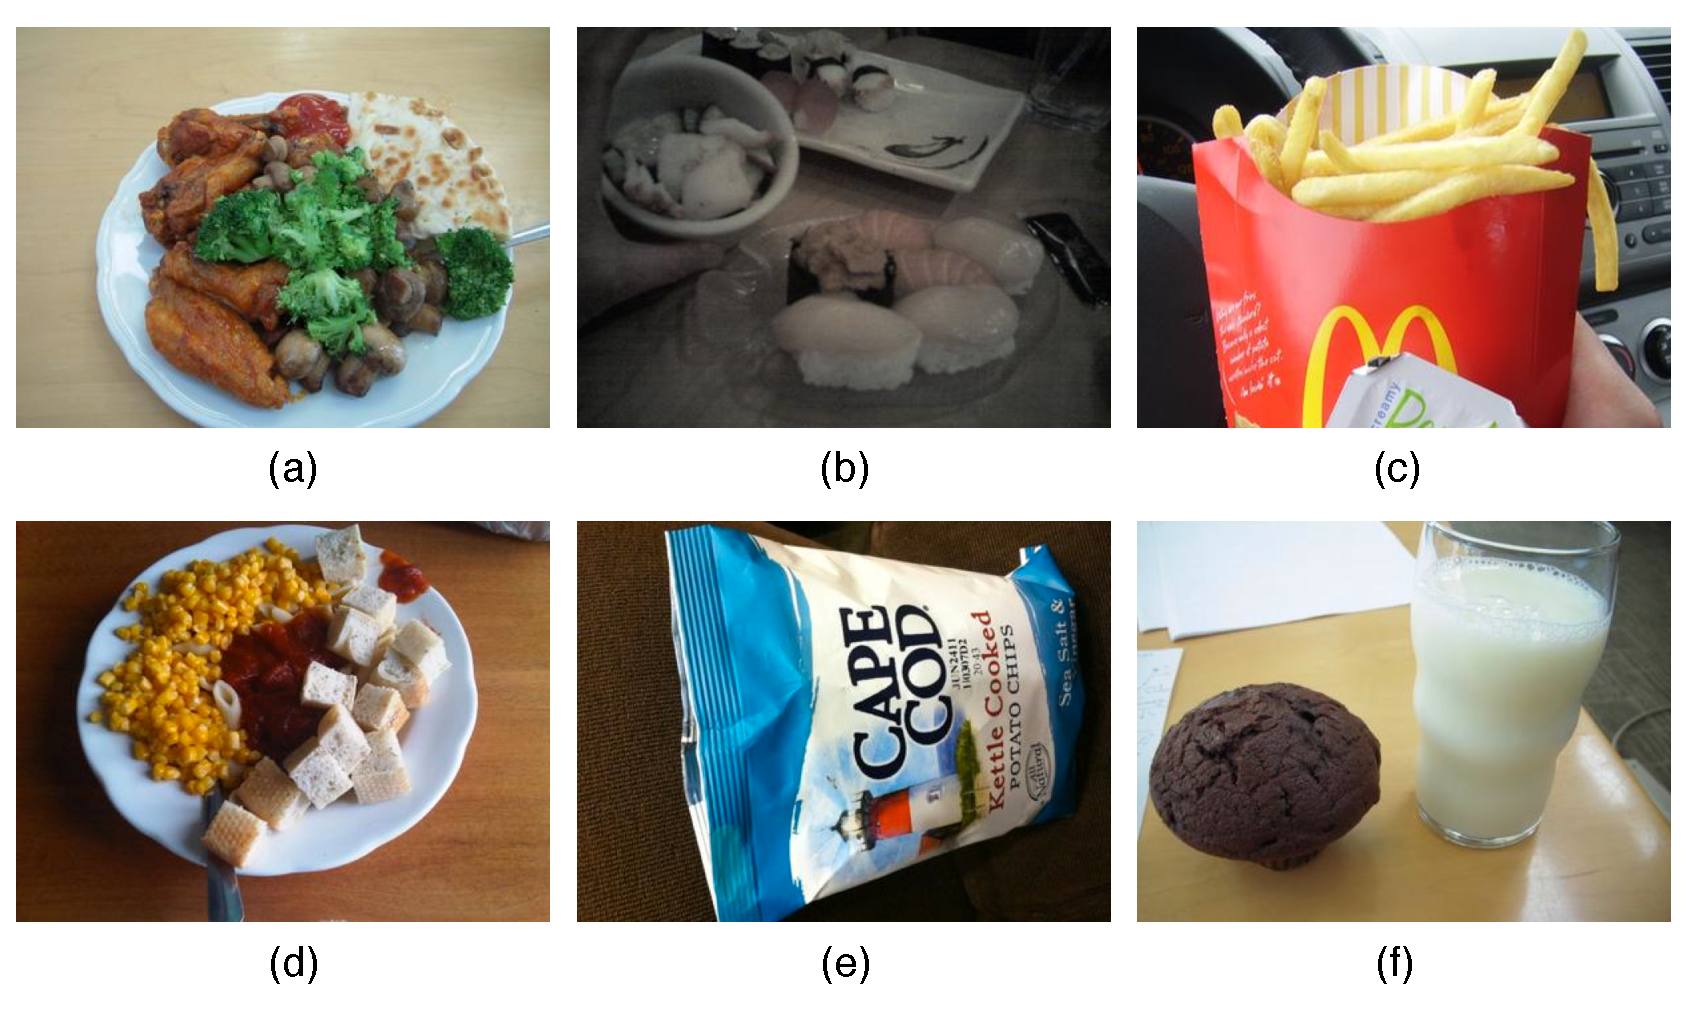
\includegraphics[width=\columnwidth]{figs/userphotos.pdf}
   \caption{Example user photos.  PlateMate handled (a) - (c) well, while (d) - (f) caused problems.  In (d) the pasta with sauce in the middle was hard to see; in (e) there is no sense of scale to determine the size of the bag; and in (f) the type of milk is unclear.}
   \label{fig:userPhotos}
\end{center}
\end{figure}

\subsubsection{Findings from the Initial Interviews}
Our pre-interviews with participants confirmed that existing methods of logging food are cumbersome. All but one of the 10 had tried logging their food at some point, but most gave up after a few days or weeks. Only two participants still tried, and neither reported doing so consistently or reliably. They recalled their attempts to keep track of food as ``annoying,'' ``inconvenient,'' and ``tedious.'' One subject recalled six separate failed attempts, each lasting just a few days. Some reported success when they were required to log for athletics or class projects, but recording lapsed when those commitments ended.

Despite these challenges, participants found nutritional information valuable. Eight participants reported looking at nutrition labels on packaged foods. Several reported looking up new foods out of curiosity. One participant reported revelations like ``Oh wow, that's a lot of calories in dressing,'' and another now dilutes her juice with water after discovering how much sugar it contains.

% I think this paragraph and the next can be cut. --EH
%Subjects acknowledged that finding this information is more difficult when foods are not packaged with labels. When eating prepared meals, especially in restaurants, they sometimes guessed crude nutrition estimates. Many had some background nutrition knowledge, which gave them a rough idea of the protein, fat, and carbohydrate levels of different kinds of foods. %One subject explained, ``When I'm at Subway getting a sandwich, I know if I get turkey and no cheese and a vinaigrette, it's better than getting the works because there's less fat.''

%Others relied on heuristics or rules of thumb for healthy eating, which don't require any systematic knowledge. Two subjects spoke of color variety and drawing from different food groups, emphasizing ``greens'' on the plate. Another spoke of eating ``like mom taught you.'' Others learned from their feelings after eating. One subject explained, ``I feel more grossed out at the fast food spots.''

\subsubsection{Exit Interview Reactions}
We asked all ten participants their preference between using PlateMate for automatic estimates and logging manually (by any method). Seven participants said they would prefer using PlateMate in the future, citing its ease of use and the convenience of ``having someone else do that for me rather than guess myself.'' One subject explained, ``My answers were closer to guesswork; this felt more like science.'' The three subjects who did not prefer PlateMate felt that they could not trust it or that the process of taking photos and correcting the estimates was too cumbersome.

Subjects were divided in their perceptions of PlateMate's
accuracy. Seven of 10 found the answers at least as good as their
own and of these four found PlateMate's estimates to be more accurate than self
reports.  After seeing his
own estimates and PlateMate's for the same meals, one subject said the
exercise ``confirmed my suspicions that you guys were more accurate
than I was. The tendency is always to say `oh, I didn't have that
much.''' Three others found their own estimates and PlateMate's
basically equivalent.

The other three subjects all found PlateMate less accurate than their
own estimates. One said that PlateMate's answers were close, ``like
$80$-$90\%$, but not perfect. I want to be sure.'' Another still
preferred PlateMate even though she could not fully trust its
results. She explained, ``For some people if it's not perfect they'll
never use it. But for me it was great...Even if it is only half of
them correct, that is fewer I have to enter manually, and the happier
I am.'' Another user disagreed, feeling that it took more effort to
correct PlateMate estimates than ``do it right myself the first
time.''

In total, seven users said that PlateMate required less effort than
manual logging, which most of these users considered unpleasant and
tedious. They called it ``annoying'', ``boring,'' and ``not
excruciating but not insignificant either.'' These participants said
PlateMate was ``definitely easier'' and ``much simpler,'' concluding
that it ``definitely saves me time and effort.'' They also found
receiving the results exciting. One user explained, ``it was more
fun...I got the email, and my friend was like, `Oh! Do we get to see
it now?''' Another was discouraged by the difficulty of manually
estimating portions, so she found it ``really helpful to have someone
else do that for me rather than guess myself.''

\subsubsection {PlateMate Performance}

Next, we analyze PlateMate's performance on photographs collected by
our users.  We wanted to investigate the system's robustness given a
broad variety of meals and realistic variations in photograph quality.
Ideally, the PlateMate estimates and manual logging data from the user
study could be compared to ground truth to determine accuracy, but
such data were clearly not available.

Instead, we first looked at the differences between participant and PlateMate estimates.  Comparing results from $112$ photos for which we had both participant and PlateMate estimates, we found the two sets of results to be positively correlated ($r^2=0.62$, $p<.0001$). PlateMate's estimates were slightly higher than participants', with a mean difference of $+41.0$ calories (median $+18.8$) or $+11.5\%$ that was not statistically significant (Wilcoxon $z=686$, {\it n.s.}). 

To gain further insight into relative accuracies of PlateMate and our participants, we presented 50 of these photographs together with both sets of nutritional estimates to 4 professional nutritionists.  The nutritionists worked in pairs.  Each pair was presented with a photo and two sets of numbers representing total calories, protein, fat, and carbohydrates.  One of these sets came from a participant and one from PlateMate, and the experts were blind to the source of the data.  They were then asked to pick the more accurate set, taking as much time as necessary and using any necessary tools and references.  The dietitians in each pair were allowed to talk to each other and could choose to agree on one data set as more accurate, disagree, or say they were unable to pick one data set as more accurate.  

%To verify the reliability of using human experts for this task, interspersed with the 50 photos from the user study were 10 photos from the ground truth study with one data set for the ground truth nutrition data and one an arbitrary error between 20\% and 50\% off of ground truth (the errors included both under- and overestimates).  Unfortunately, of the 10 ground truth photos, both pairs of dietitians picked the correct ground truth data set 50\% of the time, and we observed no bias toward either over- or underestimates.

Of the 50 user study photos, the first pair could not decide which set of nutritional estimates was more accurate in 5 cases and the second pair could not in 12 cases.  Out of the decisive photos, PlateMate data was selected as more accurate $44.4\%$ and $47.4\%$ of the time by the two pairs. These results suggest that neither method was obviously more accurate, especially since nearly half ($49.2\%$) of photos had estimates within 100 calories of each other.

% Do we need this paragraph? We're undecided. - JN
When disagreements did happen, PlateMate's estimates were larger $63.5\%$ of the time. This is consistent with our finding in the first study that PlateMate slightly overestimates and prior research that suggests a strong bias in manual recording towards underestimation.~\cite{pikholz2004under,goris2000undereating}.  PlateMate's estimates for daily energy intake were $+229.8$ calories higher than self-reports on average, a difference equivalent to four Oreo cookies every day.

\subsubsection{Error Analysis}
Many of the errors seen from the user study results were similar to those already discussed from the ground truth study, but some new issues emerged.  In measurement, we saw difficulty estimating portions when extreme close-up photos were taken with no sense of scale.  Turkers could not agree if a bag of potato chips (Figure~\ref{fig:userPhotos}) was a portion or large bag.  Scale was also a problem in identification: a small tangerine was identified as a larger orange.  Other identification errors occurred when foods with nearly correct names but vastly different nutrition were selected, like ``grapefruit juice'' and ``juice concentrate,'' which has eight times the calories. One Subway chicken sandwich was identified as ``Subway Roasted Chicken Patty,'' which could be interpreted as the whole sandwich but in fact just contained the chicken.

Human errors during manual logging mostly occurred when participants forgot to log a certain food.  In photo (f) of Figure~\ref{fig:userPhotos} the participant only recorded the milk and forgot to log the muffin, which represented most of the photo's calories.  In a photo of french fries, a participant forgot to record the dipping sauce next to the fries.  Similar errors occurred when participants sought to simplify their recordings to save time.  One subject ate a bowl of several types of fruit but recorded the entire bowl as raspberries, while PlateMate correctly identified each fruit.

\subsubsection{Cost and Wait Times}
During the course of both evaluations we analyzed 262 photos using PlateMate, generating 1,553 HITs that were assigned to 199 total Turkers 4,332 times.  The average cost of a single photo was \$1.40.  The mean time to complete analysis was 94.14 minutes, with 73\% of photos completing in less than 2 hours and all photos completing in less than 6 hours.
